\section{Course Pages}
\subsection{Overview}
The course pages are a crucial component of any learning management system. It is the place where students and academics mainly interact with the LMS and acts as the centralised page in which other components are linked, for example the lectures, tutorials and quizzes. 
The course pages also includes the course content and course outline pages. The course content is the page where slides, tutorial questions and notes are found and the course outline is where the crucial course outline and learning outcomes of the course are found.
These pages offer other bonus functionality such as widgets which will be discussed in further sections.

\subsection{Pages}
The main 3 pages that the course pages will encompass are:
\begin{itemize}
    \item The main dashboard/page
    \item The course content page
    \item The course outline page
\end{itemize}

\subsubsection{Main Dashboard/Page}
\begin{figure}[h]
    \centering
    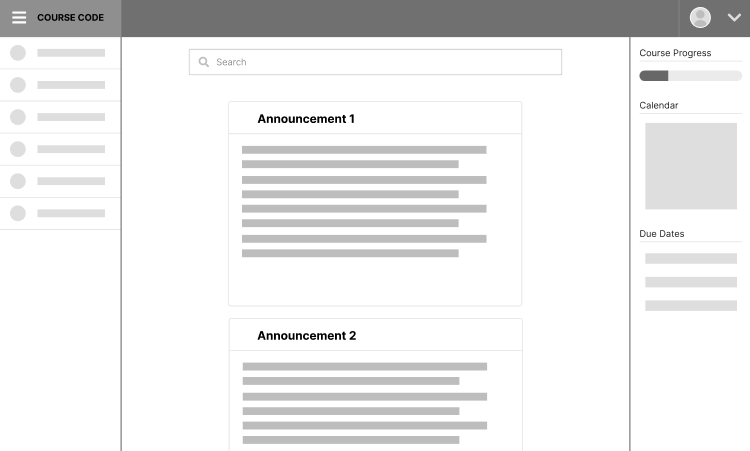
\includegraphics[scale=0.5]{course-pages-main}
    \caption{The main dashboard/page within the course.}
\end{figure}
\begin{figure}[h]
    \centering
    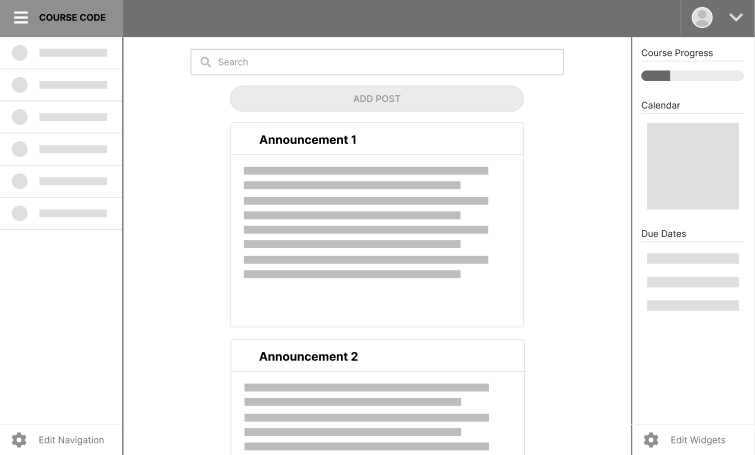
\includegraphics[scale=0.5]{course-pages-main-admin}
    \caption{The administrator view of the main dashboard/page.}
\end{figure}
The main dashboard/page is the centralised aspect of the course pages.
This page provides users with somewhat of a default home page for a particular course.
Within this page there will be a main dashboard/feed, a sidebar which links users to different aspects of the course and customisable widgets which provide further functionality. 

The main dashboard/feed acts as the display of all announcements by administrator and academics. Administrators and academics are able to create announcements in which all users in the corresponding course will be notified.
The specifics of how the notifications are to be discussed in the notifications component catergory and will not be considered here. 
Announcements are crucial to a course as they provide an efficient method of communication between administrators, academics and students/users.
Users creating announcements will be able to attach files and links to better improve the usability of the planned LMS.
Within each announcement, users will also be able to create comments.

The sidebar for the dashboard page is a component within the page that provides the user with the ability to navigate through other aspects of the LMS.
Currently the components that will be linked in the sidebar are (this is subject to change):
\begin{itemize}
    \item Course outline;
    \item Course content;
    \item Topic Tree for the course;
    \item Course Forum;
    \item Lectures and Tutorials; and,
    \item Assessments (Quizzes/Polls).
\end{itemize}

The final component of the main page are the customisable widgets. These widgets offer more extensive usability and utility for users of the LMS.
Some features that they offer are a course progress tracker and a calendar for users to view course due dates. 
These widgets are planned to be customisable such that they can be placed in different positions and can also be toggled on or off.
These widgets could also be developed by third party developers willing to create extensions to the functionality of the LMS.

\subsubsection{Course Content Page}
\begin{figure}[h]
    \centering
    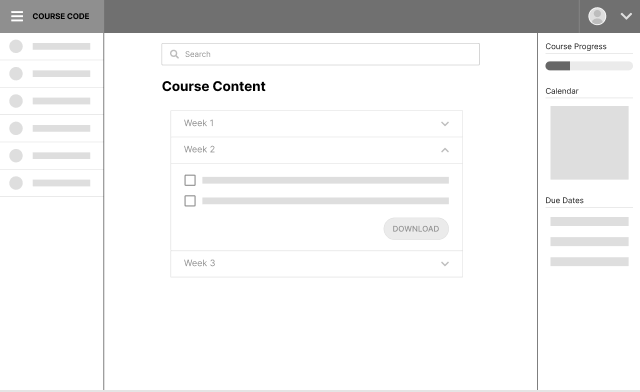
\includegraphics[scale=0.5]{course-pages-content}
    \caption{The course content page within the course.}
\end{figure}
\begin{figure}[h]
    \centering
    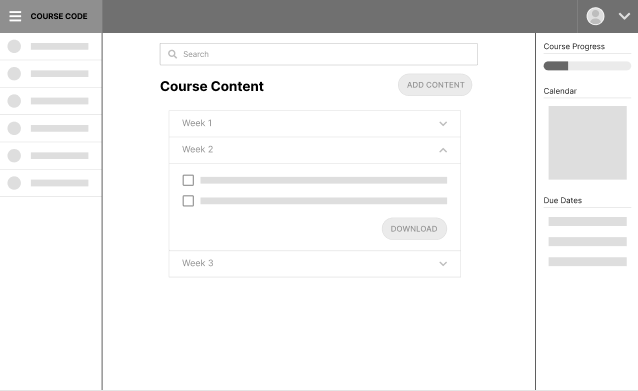
\includegraphics[scale=0.5]{course-pages-content-admin}
    \caption{The administrator view of the course content page.}
\end{figure}
The course content page is the area in which content is uploaded by administrators or academics and downloaded, viewed or completed by students.
The course content page will contain content from the topic tree and will be catergorised accordingly. 
One assumption made for the topic tree component is that the topic tree will be utilised as a database which stores content that can be utilised in courses.
Course administrators would have the ability to select which content to import into the course content page. 
Another assumption is that the content within the topic tree will be catergorised and this catergorisation will then be imported into the page.
For example if the administrator had catergorised content in the topic tree by weeks, then importing it within the course pages will retain the catergorisation method.
This is to ensure flexibility and usability for administrators and users of the LMS.
Course content involves the topics that will be stored within the topic tree. This can range from lecture slides, tutorial questions, lecture recordings an even quizzes and assignments. 


\subsubsection{Course Outline Page}
\begin{figure}[h]
    \centering
    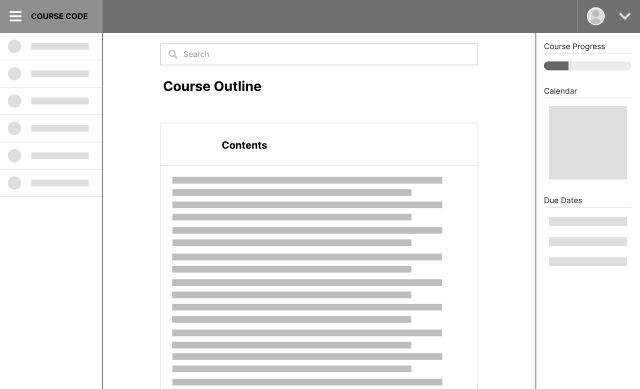
\includegraphics[scale=0.5]{course-pages-outline}
    \caption{The course outline page within the course.}
\end{figure}
The course outline page is where administrators are able to display the course outline for the particular course. 
The course outline for a course is a crucial aspect that is required for courses so that students and administrators can view the plan and outcomes of the course.
This page will act as the primary page for users to view the course outline of the course. 
Administrators will have the ability to import the course outline their files and thus be able to edit it.

\subsection{Requirements}
The requirements and use cases for the course pages are outlined below. These are subject to change as further developments within the project proceed.
These features are prioritiesed using the MoSCoW method which assists with identifying the order to implement requirements.
It contains the following catergories:
\begin{itemize}
    \item \textbf{Must have} - vital features that are critical to the basic functionality of a project.
    \item \textbf{Should have} - important features that aren't critical but add to the basic functionality of a project.
    \item \textbf{Could have} - desired features that aren't necessary to the overall project but can provide a better user experience.
    \item \textbf{Won't have} - low-priority features that likely won't be able to be completed in the given time-frame.
\end{itemize}

\subsubsection{Functional Requirements}
\begin{enumerate}
    \item Users can click on the links in the sidebar to be directed to the corresponding component (Must have)
    \item Users can view the announcments within the dashboard (Must have)
    \item Users can view the course content (Must have)
    \item Users can view the course outline of a course (Must have)
    \item Administrators of the course can create announcments within the dashboard (Must have) 
    \item Administrators can add course content into the page by selecting content from the topic tree (Must have)
    \item Users can make comments on announcments (Should have)
    \item Administrators can upload the course outline onto the course outline page (Should have)
    \item Users can download the course content (Should have)
    \item Administrators can edit the sidebar to change what components are linked (Could have)
    \item Course content is catergorised based on how the content is catergorised in the topic tree (Could have)
    \item Administrators can edit the announcements made in the dashboard (Could have)
    \item Users can intereact with widgets to enchance their experience with the LMS (Could have)
    \item Users can toggle on or off specific widgets (Could have)
\end{enumerate}

\subsection{Timeline and Milestones}
\begin{figure}[h]
    \centering
    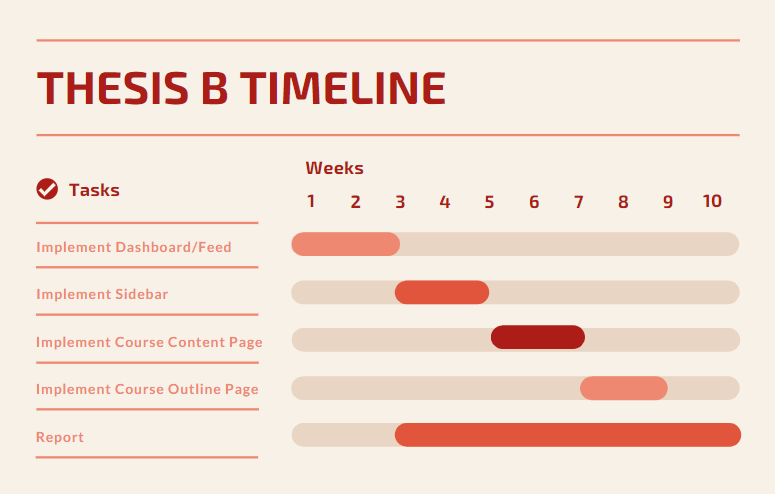
\includegraphics[scale=0.5]{thesisB-course-pages}
    \caption{Thesis B timeline.}
\end{figure}

\begin{figure}[h]
    \centering
    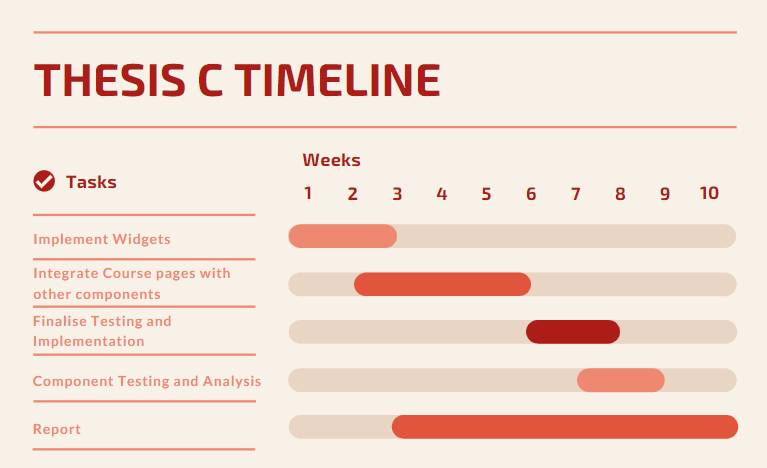
\includegraphics[scale=0.5]{thesisC-course-pages}
    \caption{Thesis C timeline.}
\end{figure}
This section will outline the timeline and milestones for the course pages.
Thesis A primarily focused on the analysis of other competitors in the literature review and the planning of features within each component in Thesis B and C.
Thesis B will focus on the implementation of the course pages as it is a crucial component that will be utilised in other components.
Thesis C will focus on the integration of the course pages with other components, such as the topic tree, forums, assessments, lectures and tutorials.
This term will also finalise all testing, analysis and evaluation of the LMS.

The major milestones for the course pages feature also highlight specific points within the project that will convey important achievements to be completed.
The important milestones for the course pages are:
\begin{enumerate}
    \item Complete Course Dashboard/Feed Page
    \item Complete Course Content Page
    \item Complete Course Outline Page
    \item Integrate Course Pages with other LMS components
    \item Final Analysis and testing of LMS
\end{enumerate}

\subsection{Evaluation}
The evaluation of the course pages will depend on a set criteria.
This criteria is proposed as followed:
\begin{itemize}
    \item Performance - Whether the course pages are fast and responsive;
    \item Accessibility - Can a wide array of users use the course pages easily;
    \item UI/UX - Is the feature easy to use and attractive; and,
    \item Errors - Is the feature bug and error free.
\end{itemize}

